\section{Introduction}

The memory management has a significant performance impact on the performance of applications, which could lead to as large as $9.7\times$ performance difference when an application is installed with different allocators, as shown in Figure~\ref{fig:motivation}. Figure~\ref{fig:motivation} evaluates the performance of five applications from two popular benchmark suite, PARSEC-2.0~\cite{} and Phoenix~\cite{}, with the default Linux allocator (Glibc-XXX), TCMalloc-2.2, jemalloc-4.2.0, and Hoard-3.11. The figure shows that choosing a different allocator may cause the performance difference between 32\% faster to 9.7$\times$ slower.   

\begin{figure}[!ht]
\centering
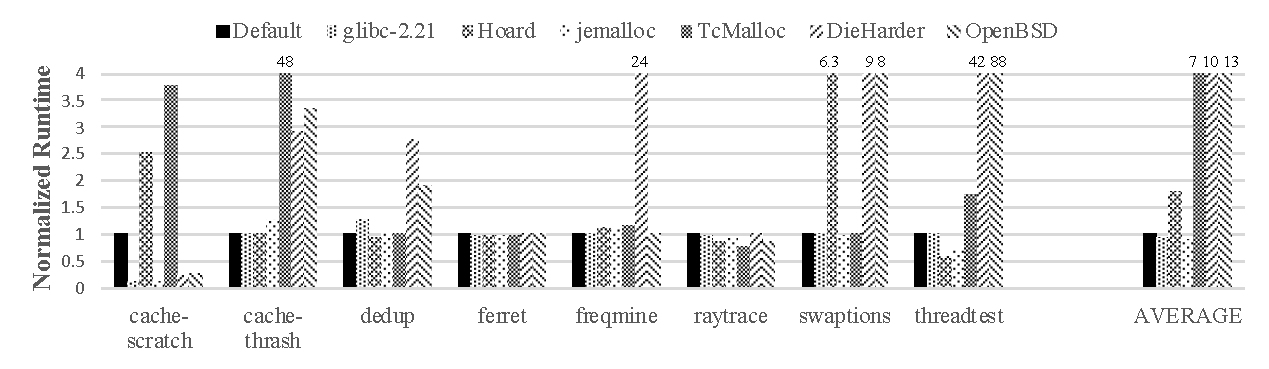
\includegraphics[width=3.3in]{figures/motivation}
\caption{Performance with Different Allocators\label{fig:motivation}}
\end{figure}

Facing with this vast performance difference of different allocators, programmers may want to choose an appropriate allocator for their applications, in order to maximize the performance potential. From the point view of allocators designers, it is extremely helpful to know the underlying reason of the performance slowdown (or speedup) of a specific version of an allocator, so that they could further improve their design. Both of their targets could be satisfied with an allocator profiler.  

However, there is no such profiler to the best of our knowledge. Existing profilers, such as mprof~\cite{Zorn:1988:MAP:894814}, TCMalloc Heap Profiler~\cite{tcmalloc-profiler}, CLR profiler~\cite{lupasc2014dynamic} or others~\cite{hirotaka2003developing}, typically focus on memory allocation behavior of applications. For instance, mprof integrates the memory allocations based on the callstack~\cite{Zorn:1988:MAP:894814}, while TCMalloc Profiler could report program sites with a large number of allocations, locate memory leaks, and report heap usage of any time~\cite{tcmalloc-profiler}. General profilers, e.g. gprof~\cite{}, and perf~\cite{}, are not suitable for profiling memory allocators as well, since they typically cannot differentiate the behavior caused by allocators or applications. 
 
The lack of a general profiler typically makes  allocator developers design their custom profilers every time, which causes the waste of human resources each time. Also, the nonexistence of the allocator profiler makes the quantitative comparisons of different allocations very difficult. Existing comparisons~\cite{Barroso:1998:MSC:279358.279363, Masmano:2006:CMA:1167999.1168012, ferreira2011experimental}, mostly just evaluate the performance of a set of applications. 
%Even if the comparisons could identify an allocator cannone allocator has the best performance on average, 
These comparisons could not pinpoint the underlying reason behind that for the good or bad performance. 
%Therefore, they could not guide the choice of allocators well, since the best performance on these applications may not be good for a specific applications. 
%Even if they find out that one allocator is not good at the performance by running a serial of applications, they cannot further pinpoint what issues inside the allocators. Therefore, they cannot guide the allocator designer to further fix the issues inside, or prevent such issues in the future design. 


This paper, \MP{}, designs a general profiler that profiles allocation/deallocation behavior of allocators. \MP{} focuses the following attributes of the allocator: performance overhead, memory overhead, scalability, and applications friendliness, which covers important attributes of evaluating an allocator. 

For performance overhead, \MP{} focuses on the following items: 


Since memory overhead can be caused by multiple factors, such as metadata overhead, alignment overhead (internal fragmentation), and memory blowup. Memory blowup is defined as ,. 

For scalability, \MP{} not only focuses on the potential bottleneck within the user space, but also includes the potential bottleneck caused by the allocator. Programmers have identified one particular performance bottleneck of applications, such as dedup issue. 
It won't cause the . 

\MP{} also aims to answer whether an allocator is friendly to the applications or not, such as . . 


   


MallocProfiler will serve two purposes. 
(1) This will be utilized to get the allocator related parameters. 

(2) We will be able to identify whether the performance problem is caused by the memory allocator. We could actually divide the overhead to the overhead of allocator or the overhead of applications. 
Therefore, we could identify the root causes and not always blame for the application writer. 



 

However, the memory allocator itself has not got sufficient attention that it should reserve to. 
For instance, there is no an dedicate the allocator profiler that can be utilized for identify the allocator's behavior.

Having this profiler will serve three purposes. First, it will help the designers and developers that could discover the issues of memory allocators, without the need of porting or developing the profiler for a specific allocator. Second, it helps programmers to determine whether the performance issue is coming from the memory allocator. Third, it will help users to choose the best memory allocators that is suitable for a specific applications, if there are multiple choices available. 

 Linux, TCMalloc, Jemalloc, Hoard, OpenBSD, DieHarder. Then shows the internal reason of why some are slower than others. 

We may choose two general-purpose allocators and two secure allocators. Then we know why secure allocators are slower, currently. 

The general idea is to understand performance, memory, and scalability of different allocators, while providing some evidence of allocator. During the design of allocator, we usually need to understand the inherent reason. The difficulty is how to collect the information without changing the specific allocator. That is, how to design a general allocator profiler, which can help assist the analysis of different allocators. 

We will work on the allocator profiling to understanding the performance, memory and scalability of memory allocator. We may  memory related those system calls. How long it spent on the memory allocation and deallocation, using rtdsc, which can be caused by long memory allocation time? How much of objects has been re-utilized? How is the memory blowup, what is the memory consumption and how much has been allocated? Can we know lock contention of memory allocation, maybe we could monitor the lock usage, just as SyncPerf, and identify that lock acquisitions are  waiting during allocation? Can we identify is there inter-objects cache contention on these objects? If yes, that is the possible example of these allocators.  

What are the design goals of \MP{}? 

\MP{} needs to be general to different memory allocators, which requires no change of the code at all even when connecting with different allocators. The first target is transparency, which should not require the changes of allocators, if the allocator is working as a dynamic library. 

Second, \MP{} should be able to identify the issues of different allocators. 


Overall, it will three categories. Also, we would like to know some internals of inside. 

Performance overhead? Why it is slow, due to memory management itself, lock contention, or too much effort on system calls. Can we use the flame figure or block figure? 

Memory overhead? Whether this allocator will utilize a large amount of memory? How much it spent on the management itself, how much it can not fully utilized?  

Maybe we should add the PMU sampling to this project, so that we can know about whether the project are helpful on the performance? Whether they introduce the false sharing issue? whether they are good in NUMA situation? 


About NUMA stuff, maybe we could use PMU to check whether the allocator has a larger performance overhead? 

How much is running on a different core? But the question is how to know this? 

Then maybe we could use it to explain the performance difference of different allocator. 


\begin{comment}

Dynamic memory management plays an important role in the performance of applications, especially on multithreaded programs. 
For performance related to memory uses, some work focuses on improving existing memory allocators. Some focuses on a better memory layout among different elements of the same data structure. 
But there is little work that focuses on the improving the performance by changing the behavior of memory allocations and deallocations. 

\HeapPerf{} tries to identify some places inside applications that can introduce the performance problems. These problems can be solved by changing the behavior of memory allocations, without using the new memory allocator. 
These problems are rarely investigated in the past. The most closest work related to this is to simply record the placement with excessive allocations. However, excessive allocations is a total class of the problems that are investigated in this paper, but the existing work fails to present any detailed idea on the following problems: whether all these excessive memory allocations can be reduced? whether they can improve the performance? how to reduce that? These questions requires highly expertise and large amount of manual effort. Instead, \HeapPerf{} presents more useful idea on these questions, and hope to guide programmers, even non-experts, to solve these problems easily. 

We observe three different patterns that can cause performance problems, or called as anti-patterns~\cite{}. 

The second type is shown as Figure~\ref{}. In this example, there are a number of memory allocations that will allocate small amount of bytes for each one. More particularly, these allocations are inside the same loop, and have the same size. Unfortunately, memory allocators will not precisely allocate the specified size of objects. For example, the \texttt{glibc} allocator will allocate 32 bytes as long as the required size is between 4 bytes and 24 bytes. Based on the explanation of Hoard~\cite{Hoard}, this method helps to manage small sizes of different objects, without introducing too many external fragmentation. However, this also introduces a significant problem on cache inefficiency, since only less than 13\% cache is actually utilized, which can introduce around $8\times$ performance slowdown comparing to the code listed in Figure~\ref{}. 


The second type is shown as Figure~\ref{}, there are a number of unnecessary memory allocations and deallocations. By moving the placement of allocations to outside the loop, we can significantly improve the performance by reducing the overhead related to memory allocations and deallocations. 

The third type is related to the uses of heap variables or stack variables. Some excessive heap objects, if they are turned into stack variables, will have large performance benefit. Comparing to heap objects, the overhead of memory allocations and deallocations can be largely reduced if using stack variables. Also, the stack is typically locate inside the cache, which will have lower access latency. Also, stack variables will have exact size, without the addition of metadata and huge alignment. 
\todo{Whether those variables have been touched only very few times, typically should be putted into the heap objects since they may cause the in-efficient cache utilization as well}.  
 


Heap memory related performance bugs can be from the following categories, if only think about applications. 

\begin{itemize}
\item: Too many allocations and deallocations. The total run time spending in memory allocation and liberation may take up to 30\% execution time\cite{1190248}. 

\item: Too many memory uses: this can actually affect the performance when there are too much memory that has been allocated but not used. This can be caused by memory leaks or too late de-allocation. \todo{Most existing tools focus on the memory leak, but whether there are some tools that can uncover delayed-deallocation?}  

\item: 
\end{itemize}


What we can do for heap memory management?

First, we can point out the unnecessary memory allocations and deallocations. For example, we can malloc a large object, and then assign to different small projects. Some of them may be called inside the internal level of loop functions, we can move up to external loop level. 
By reducing unnecessary memory allocations, we expect to improve the performance. 

Second, we can give a statistics on the life-span of objects. Whether we can find out some problems inside? For example, we can use stack variables instead of heap if some objects are too short-lived, or mostly inside a function call. 

Third, we can actually give the statistics on each callsite. Some callsites may have larger number of allocations. 

Can we evaluate the performance related to heap allocations? For example, how much time is spending on memory allocation. 
We can approximate the time of spending on each allocation. Then we can attribute the time to different statements, just similar to gprof. Then maybe it is obvious that we can reduce the overhead by reducing the memory allocations. Then it is possible that a separate paper by using the 


In the end, although not every interested, it is to check the overhead of every memory allocation on each popular memory allocation. Thus, pointing out that the memory allocation actually should pay attention to the level of stacks. Thus, it is possible that we can design a new memory allocator by reducing the level of memory allocation. This is a reverse to HeapLayer. It is great to have an survey paper on this:

A. How is the overhead of memory allocation in large applications? How we can evaluate it? 
B. How is the overhead that comes from memory management? We evaluate this on some popular benchmarks. 
C. Whether the overhead comes from different cache uses? or other things. 
D. It will shed a light whether we need to re-design the memory allocator. 
It will be a perfect paper for ICSE or SC.

How we can evaluate the cache friendliness of memory allocators? 
For instance, how much memory will be reutilized immediately? If one direct use will be one point, then how many score of different allocators. 

Also, how much of memory blowup? 

%%%%%%%%%%%%%%%%%%%%%%%
% Possible solutions:
% (1) We will check the malloc and free are allocated in sequence. For example, we are always doing the malloc(8) and free(8) in sequence. Given the number of these allocations is large. Then it is much possible that it is a problem. However, it can be a problem for the performance reason. But we can basically maintain a stack that maintains five possible allocations. 
%% Should we just use a two-phase solution? That is, we can use a hash-table to identify different allocation site with their memory uses: how many times for memory allocations? How many times for related free operations? If there are a lot of memory allocations that are not freed, then it is possible a memory leak. We could also identify whether those memory are actually touched or not by using the watchpoint mechanisms? Also, we may try to check whether memory allocation are in the same sequence, for example, alloc-free-alloc-free, and with the same size. If yes, then it is possible that is unnecessary memory operations. 

%%%%%%%%%%%%%%%%%%%%%%%%%
Typically, I think that mtrace utilizes 

Can we check the example of malloc-free situations?
Can we base on a ``anomaly detection'' but.  
I guess that the memory will be freed before the next allocation. If not, then there is high probability of leaking. If memory allocated is on the same site, 
	
\end{comment}
 
\subsection*{Contribution}

This paper makes the following contributions. 

\begin{itemize}
\item It proposes the first general profiler--\MP{}--to profile different memory allocators, without the change of memory allocators or allocations. \MP{} focuses on the allocation behavior of allocators, instead of focusing on applications.  

\item \MP{} can not only pinpoint the major issues inside the implementation of memory allocators, such as performance, memory, and scalability issues, but also could quantitively pinpoint some cache or page utilization issues of allocators. 

\item This paper performs extensive experiments on multiple memory allocators with a large number of allocations. It pinpoints the reason of the performance or memory issues latent in existing allocators. It also provides an experimental reasons of different allocators in general.  

\end{itemize} 

\subsection*{Outline}

The remained of this paper is organized as follows. Section~\ref{} discusses the overall design purpose of \MP{}, and Section~\ref{} presents the detailed implementation. Section~\ref{} shows the results of experiments on different allocators using \MP{}. Then Section~\ref{} discusses related work in this field, and Section~\ref{} concludes this paper. 